\chapter{Tao Initialization}
\label{c:init}

\tao is customized for specific machines and specific calculations
using input files and custom software routines. Writing custom software is
covered in the programmer's guide section. This chapter covers the
input files. 

In general the input files tell \tao:
\begin{example}
  1) What the "standard" variables should be.
  2) What the "standard" data is.
  3) What to plot and where to plot it.
\end{example}

\tao first looks for input files in the current directory and then
looks in a directory pointed to by the environmental variable
\vn{TAO_INIT_DIR}.

Initialization parameters are read in from a file using Fortran
namelist input. Fortran namelist breaks up the input file into
blocks. The first line of a namelist block starts with an ampersand ``\&''
followed by the block identifying name. Variables are assigned using
an equal sign ``='' and the end of the block is denoted by a slash ``/''
For example:
\begin{example}
  \&this_block_name
    var1 = 0.123   ! exclamation marks are used for comments
    var2 = 0.456
  /
\end{example}
Variables that have default values can be omitted from the block.  The
order of the variables inside a block is irrelevant.  In between
namelist blocks all text is ignored. Inside a block comments may be
included by using an exclamation mark ``!''.

Note: string variables are case sensitive.

%-----------------------------------------------------------------
\section{Beginning Initialization}
\label{s:init_global} 

The initialization starts with an initialization file named \vn{tao.init}. 
\vn{tao.init} needs to have a \vn{tao_start} namelist block with the following syntax:
\begin{example}
  \&tao_start
    lattice_file      = "<file_name>"  ! Default = this file.
    data_and_var_file = "<file_name>"  ! Default = this file.
    plot_file         = "<file_name>"  ! Default = this file.
    single_mode_file  = "<file_name>"  ! Default = this file.
    startup_file      = "<file_name>"  ! Default = "tao.startup"
    n_universes       = <integer>            ! Number of universes. Default = 1.
    startup_single_mode = Logical            ! Default is False.
  /
\end{example}
\vn{n_universes} is the number of universes to be created. The \vn{data_and_var_file}
\vn{single_mode_file}, and \vn{plot_file} files are described in the following sections.

%-----------------------------------------------------------------
\section{Lattice Initialization}
\label{s:init_lat} 

The \vn{lattice_file} variable in the \vn{tao_start} namelist is the
name of the file with the \vn{tao_design_lattice} namelist that
defines where the lattice input files are. The \vn{tao_design_lattice}
namelist has the form
\begin{example}
  \&tao_design_lattice
    design_lattice_file(i) = "<lattice_file>", \{"<parser>"\}
  /
\end{example}
\vn{<lattice_file>} is the name of an input lattice file and
\vn{<parser>} is the name of the parser to use. Possible choices for
\vn{<parser>} are:
\begin{example}
  bmad    ! For a standard bmad lattice file. This is the default.
  xsif    ! For an xsif lattice file.
\end{example}

Example:
\begin{example}
  \&tao_design_lattice
    design_lattice_file(1) = "this.lat"          ! Default: Use the bmad parser 
    design_lattice_file(2) = "that.lat", "xsif"  ! For universe \#2
  /
\end{example}

%-----------------------------------------------------------------
\section{Initializing Globals}
\label{s:globals} 

Global variables are initialized in the \vn{data_and_var_file} using a
namelist block named \vn{tao_params} The syntax of this block is:
\begin{example}
  \&tao_params
    n_v1_var_max  = <integer>   ! number of v1 data structures.
    n_d2_data_max = <integer>   ! number of d2 data structures.
    n_data_max    = <integer>   ! Total number of data points
    n_var_max     = <integer>   ! Total number of variables.
    global        = <tao_global_struct> ! global parameters
  /
\end{example}
Example:
\begin{example}
  \&tao_params
    n_v1_var_max  = 5
    n_d2_data_max = 6
    n_data_max    = 2000
    n_var_max     = 2000
    global%optimizer = 'lm'  ! Set the default optimizer.
  /
\end{example}
\vn{n_d2_data_max} and \vn{n_v1_var_max} are the maximum number of
\vn{d2_data} and \vn{v1_var} structures needed. \vn{n_data_max} is the
maximum number of datums needed and \vn{n_var_max} is the maximum
total number variables used. For a list of \vn{global} elements see
the description of the \vn{set} command in Chapter~\ref{c:command}.

%-----------------------------------------------------------------
\section{Initializing Variables}
\label{s:init_var} 

\vn{Variable}s are initialized using the \vn{tao_var} namelist. The
format for this is
\begin{example}
  \&tao_var
    v1_var%name        = "<var_array_name>"  ! Variable array name.
    default_universe   = "<integer>"         ! Universe variables belong in.
    default_attribute  = "<attribute_name>"  ! Attribute to control.
    default_weight     = <number>            ! Merit_function weight.
    default_step       = <number>            ! Small step value.
    default_merit_type = <merit_type_name>   ! Sets how the merit is calculated.
    default_low_lim    = <number>            ! Lower variable value limit. 
    default_high_lim   = <number>            ! Upper variable value limit. 
    ix_min_var         = <integer>           ! Minimum array index.
    ix_max_var         = <integer>           ! Maximum array index.
    var(i)%name        = "<var_name>"        ! Individual variable name.
    var(i)%ele_name    = "<ele_name>"        ! Element to be controlled.
    var(i)%attribute   = "<attrib_name>"     ! Attribute to be controlled.
    var(i)%universe    = "<integer>"         ! Universe to be controlled.
    var(i)%weight      = <number>            ! Merit function weight.
    var(i)%step        = <number>            ! Small step size.
    var(i)%merit_type  = <merit_type_name>   ! Sets how the merit is calculated.
  /
\end{example}
Example:
\begin{example}
  \&tao_var
    v1_var%name      = "v_steer"   ! vertical steerings
    default_universe  = "clone"
    default_attribute = "vkick"     ! vertical kick attribute
    default_weight    = 1e3
    default_step      = 1e-5
    ix_min_var        = 0
    ix_max_var        = 99
    var(0:99)%name      = "0w", "1w", "2w", "  ", "4w", ...
    var(0:99)%ele_name  = "v00w", "v01w", "v02w", "    ", "v04w", ...
  /
\end{example}

A \vn{tao_var} block is needed for each variable array to be defined.
\vn{v1_var%name} is the name of the array to be used with \tao
commands. The \vn{var(i)} array of variables has an index \vn{i} that runs
from \vn{ix_min_var} to \vn{ix_max_var}. Each variable has a name 
\vn{var(i)%name} to which it can be refered to in \tao commands. 
A lattice element name \vn{var(i)%ele_name} and the element's attribute to vary
\vn{var(i)%attribute} needs to specified. Not all elements need to 
\vn{exist} and the element names of non--existant elements should be undefined
or set to a name with only spaces in it. For those variables where
\vn{var(i)%attribute} is not specified in the namelist the \vn{default_attribute}
will be used. 


\vn{var(i)%step} establishes what a ``small'' variation of the
variable is. This is used, for example, by some optimizers when
varying variables. If \vn{var%step(i)} is not given for a
particular variable then the default \vn{default_step} is
used. 

\vn{var(i)%universe} gives the universe that the
lattice element lives in. If \vn{var(i)%universe} is not present 
\vn{default_universe} is used instead. In addition to a number 
\vn{default_universe} can have values:
\begin{example}
  "gang"     -- Multiple universe control (default).
  "clone"    -- Make a var array block for each universe.
\end{example}
With both \vn{"gang"} and \vn{"clone"} individual \vn{var(i)%universe}
may not be set in the namelist. \vn{"gang"} means that each variable
will control the given attribute in each universe
simultaneously. \vn{"clone"} means that an array of variables will be
duplicated, one for each universe.  To differentiate variables from
different universes \vn{;n} will be appended to each \vn{v1_var%name}
where \vn{n} is the universe number.  For example, if \vn{v1_var%name}
is \vn{quad_k1} then the variable block name for the second universe will
be \vn{quad_k1;2}. The default if both \vn{default_universe} and all
\vn{var(i)%universe} are not given is for \vn{default_universe} to be
\vn{"gang"}

\vn{var(i)%weight} gives
the weight coefficient for the contribution of a variable to the merit function. 
If not present then the default weight of \vn{default_weight} is used.
\vn{var(i)%low_lim} and \vn{var(i)%high_lim} give the lower and upper bounds
outside of which the value of a variable should not go. If not present 
\vn{default_low_lim} and \vn{default_high_lim} are used. If these are not
present as well then by default
\begin{example}
  low_lim  = -1e30
  high_lim =  1e30
\end{example}
\vn{var(i)%merit_type} determines how the merit contribution is calculated.
Possible values are:
\begin{example}
  "limit"       ! Default
  "target"      
\end{example}
For details on \vn{limit} and \vn{target} constraints see the chapter on Optimization.

\tao can search for the elements in the lattice to be associated with 
each variable type, Likewise, the names for data points can be automatically
generated by using the syntax:

\begin{example}
  var(0)%name = "COUNT: <name_string>###"
  var(0)%ele_name = "SEARCH: <search_string>"
\end{example}
Where \vn{<name_string>} is used in the generation of the variable name and the
hashes is replaced by the variable number in the series starting with
\vn{ix_min_var} (as an integer whose length is equal to the number of 
hashes). \vn{<search_string>} can contain the wildcards
\vn{*} and \vn{%}. For example:
\begin{example}
  &tao_var
    v1_var%name  = "quad_k1"
    default_attribute = "k1"
    ...
    ix_min_var = 1
    var(0)%name = "COUNT: Q_####"
    var(0)%ele_name = "SEARCH: Q*"
  /
\end{example}

This will search for all lattice elements whose names contain 'Q' followed
by any set of characters and will name the data elements as 'Q\_'
followed by the variable number in the v1\_var array starting with 0001. 

Variables can also be searched using the \bmad element \textit{key} attribute
using the syntax:

\begin{example}
  var(0)%name = "COUNT: <name_string>###"
  var(0)%ele_name = "SEARCH_KEY: <key>"
\end{example}
Where \vn{<key>} is the \bmad \textit{key} attribute. For example:
\begin{example}
  &tao_var
    v1_var%name  = "quad_k1"
    default_attribute = "k1"
    ...
    ix_min_var = 1
    var(0)%name = "COUNT: Q_####"
    var(0)%ele_name = "SEARCH_KEY: quadrupole"
  /
\end{example}
will search for all quadrupole elements in the lattice.


%-----------------------------------------------------------------
\section{Initializing Data}
\label{s:init_data} 

Data is initialized using the \vn{tao_d2_data} namelist block whose format is
\begin{example}
  \&tao_d2_data
    d2_data%name = "<d2_name>"    ! d2_data name.
    universe     = <integer>      ! Universe variables belong in.
                                        !   0 => all universes (default).
    default_merit_type = "<merit_type>" ! Sets how the merit is calculated.
    n_d1_data          = <integer>      ! Number associated d1_data arrays.
  /
\end{example}
For example:
For example:
\begin{example}
  \&tao_d2_data
    d2_data%name = "orbit"
    universe     = 0  ! apply to all universes
    n_d1_data    = 2
  /
\end{example}
A \vn{tao_d2_data} block is needed for each \vn{d2_data} structure
defined. \vn{d2_data%name} gives the name of the structure.
\vn{universe} gives the universe that the data is associated with. A
value of zero means that a \vn{d2_data} structure is set up in each
universe. \vn{default_merit_type} determines how the merit function
terms are calculated for the individual datum points. Possibilities
are:
\begin{example}
  target
  max
  min
  abs_max
  abs_min
\end{example}
See the chapter on optimization for more details.  

\vn{n_d1_data} defines how many \vn{d1_data} structures are associated
with the \vn{d2_data} staructure. For each \vn{n_d1_data} structure
there must be a \vn{tao_d1_data} namelist which has the form:
\begin{example}
  \&tao_d1_data
    ix_d1_data         = <integer>      ! d1_data index
    d1_data%name       = "<d1_name>"    ! d1_data name.
    default_data_type  = <type_name>    ! Eg: orbit:x, beam_energy, etc...
    default_weight     = <number>       ! Merit function weight.
    ix_min_data        = <integer>      ! Minimum array index.
    ix_max_data        = <integer>      ! Maximum array index.
    data(j)%name       = "<data_name>"  ! Data names.
    data(j)%data_type  = "<type_name>"  ! Eg: "orbit:x", etc.
    data(j)%ele_name   = "<ele_name>"   ! Lattice element names.
    data(j)%ele2_name  = "<ele2_name>"  ! Lattice element names.
    data(j)%merit_type = "<merit_type>" ! Sets how the merit is calculated.
    data(j)%meas_value = "<number>"     ! Datum "measured" value
    data(j)%weight     = "<weight>"     ! Merit function weight.
    data(j)%good_data  = Logical        ! Valid for optimization and plotting?
  /
\end{example}
For example:
\begin{example}
  \&tao_d1_data
    ix_d1_data        = 1 
    d1_data%name      = "x"  
    default_weight    = 1e6
    ix_min_data       = 0
    ix_max_data       = 99
    data(0:)%name     = "0W",      " ", "2W", ...
    data(0:)%ele_name = "DET_00W", " ", "DET_02W", ...
  /
\end{example}
Alternatively one can specify a datum in a single line. For example:
\begin{example}
  \&tao_d1_data
  ...
  data( 1) = ' '  'beta:x'  'Q09_1'  'Q16_1'    'max'    30   0.1   T
  data( 2) = ' '  'beta:y'  'Q09_1'  'Q16_1'    'max'    30   0.1   T
  data( 3) = ' '  'floor:x' 'end_arc' ' '       'target'  3   0.01  T       
  ...
  /
\end{example}


\vn{ix_min_data} and \vn{ix_max_data} give the bounds for the
\vn{data(i)} structure array that is associated with the \vn{d1_data}
structure. \vn{data(:)%name} gives the names of the data points and
\vn{data(:)%ele_name} gives the lattice element names associated
with the data points.  If elements in the \vn{data} array do not exist
the corresponding \vn{var%name} and \vn{data%ele_name} should be left
blank. Lists of names can be reused using the syntax:
\begin{example}
  data(0)%name = "SAME: <d2_name:d1_name>"
  data(0)%ele_name = "SAME: <d2_name:d1_name>"
\end{example}
For example:
\begin{example}
  \&tao_d1_data
    ix_d1_data       = 2
    d1_data%name     = "y"  
    ...
    data(0)%name     = "SAME: orbit:x"
    data(0)%ele_name = "SAME: orbit:x"
  /
\end{example}

\tao can search for the elements in the lattice to be associated with 
each data type, Likewise, the names for data points can be automatically
generated by using the syntax:

\begin{example}
  data(0)%name = "COUNT: <name_string>###"
  data(0)%ele_name = "SEARCH: <search_string>"
\end{example}
Where \vn{<name_string>} is used in the generation of the data name and the
hashes is replaced by the data number in the series starting with
\vn{ix_min_data} (as an integer whose length is equal to the number of 
hashes). \vn{<search_string>} can contain the wildcards
\vn{*} and \vn{%}. For example:
\begin{example}
  \&tao_d1_data
    ix_d1_data       = 1
    d1_data%name     = "x"
    ix_min_data      = 1  
    ...
    data(0)%name     = "COUNT: BPM_####"
    data(0)%ele_name = "SEARCH: BPM*"
  /
\end{example}

This will search for all lattice elements whose names contain 'BPM' followed
by any set of characters and will name the data elements as 'BPM\_'
followed by the data number in the d1\_data array starting with 0001. 

Data elements can also be searched using the \bmad element \textit{key} attribute
using the syntax:

\begin{example}
  data(0)%name = "COUNT: <name_string>###"
  data(0)%ele_name = "SEARCH_KEY: <key>"
\end{example}
Where \vn{<key>} is the \bmad \textit{key} attribute. For example:
\begin{example}
  \&tao_d1_data
    ix_d1_data       = 1
    d1_data%name     = "x"
    ix_min_data      = 1  
    ...
    data(0)%name     = "COUNT: BPM_####"
    data(0)%ele_name = "SEARCH_KEY: monitor"
  /
\end{example}
will search for all monitor elements in the lattice.

If \vn{data(j)%data_type} is not given and \vn{default_data_type} is not
specified then the \vn{d2_data} name and the
\vn{d1_data} name are combined for each datum to form the datum's
\vn{type}. Certain types are recognized by \tao. These are given by
Table~\ref{t:cons}

\vn{data(:)%weight} gives the weight coefficient for a variable in the
merit function. If not present then the default weight of
\vn{default_weight} is used.

%-----------------------------------------------------------------
\section{Initializing Plotting}
\label{s:init_plot} 

\subsection{Plot Window}

\begin{figure}
  \centering
  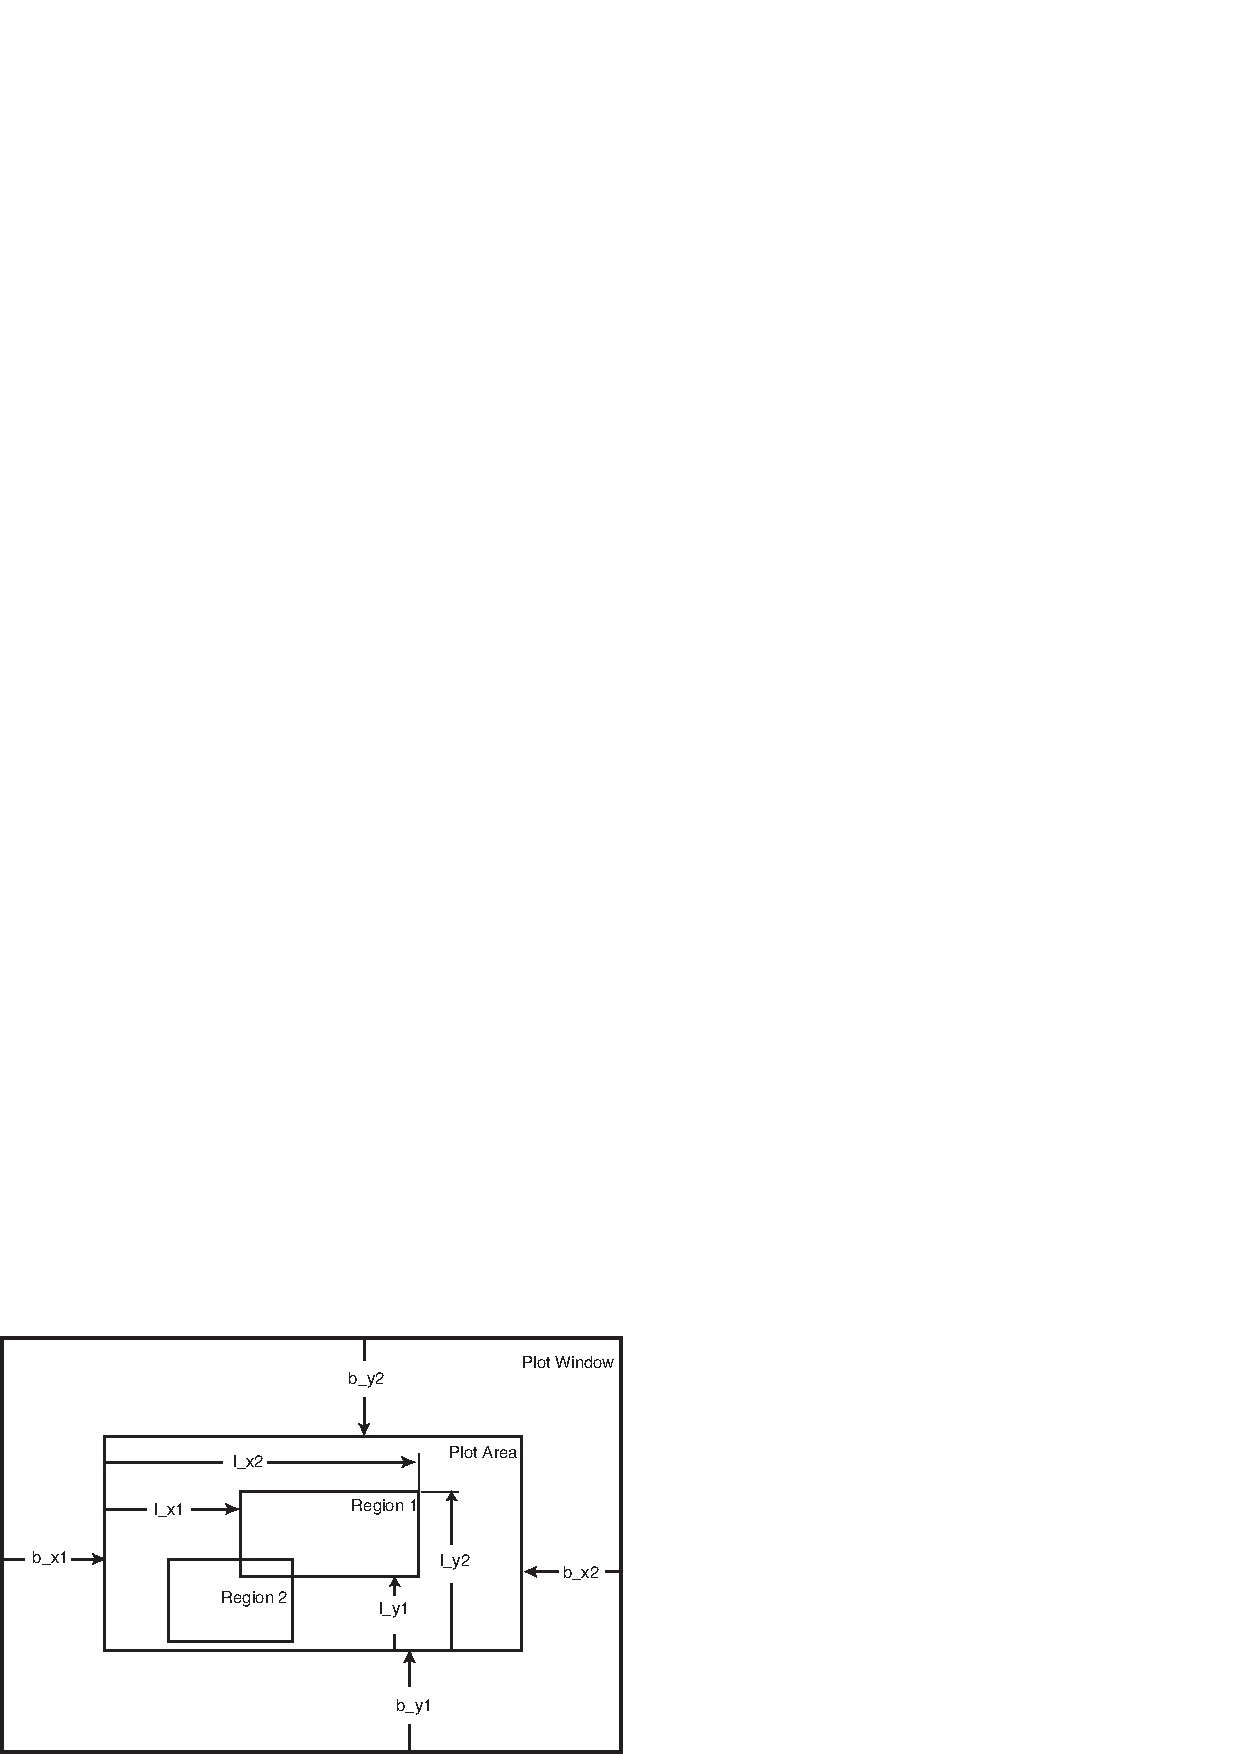
\includegraphics{plot_page.psfig}
  \caption{Regions define where on the plot page plots are placed.}
  \label{f:plot_page}
\end{figure}

Plotting is defined by an initialization file named
\vn{tao_plot.init}.  The first namelist block in the file has a block
name of \vn{tao_plot_page}. This block sets the size of the plot
window (also called the plot page) and defines the ``regions'' where
plots go. The syntax of this block is:
\begin{example}
  \&tao_plot_page
    plot_page%size        = <x_size>, <y_size>         ! size in POINTS 
    plot_page%border      = <b_x1>, <b_x2>, <b_y1>, <b_y2>, "<units>"
    plot_page%text_height = <text_height>              !height in POINTS
    plot_page%title(i)    = <string>, {<x>, <y>, "<justify>", "<units>"}
    region(i)%name        = "<region_name>"
    region(i)%location    = <l_x1>, <l_x2>, <l_y1>, <l_y2>  ! % plot area
    place(i)%             = "<region>", "<template>"
  /
\end{example}
For example:
\begin{example}
  \&tao_plot_page
    plot_page%size        = 700, 800           ! Points
    plot_page%border      = 0, 0, 0, 50, "POINTS"  
    plot_page%text_height = 12.0
    plot_page%title(1)    = "CESR Lattice"
    region(1)%name        = "top"
    region(1)%location    = 0.0, 1.0, 0.5, 1.0
    region(2)%name        = "bottom"
    region(2)%location    = 0.0, 1.0, 0.0, 0.5
    place(1)              = "top", "orbit"
    place(2)              = "bottom", "phase"
  /
\end{example}

\vn{plot_page%size} sets the horizontal and vertical size of the plot
window in \vn{POINTS} units (72 points = 1 inch. Roughly 1 point = 1
pixel). 

\vn{plot_page%border} sets a border around the the edges of the
window. As shown in Figure~\ref{f:plot_page} \vn{b_x1}, \vn{b_x2} are
the right and left border widths and \vn{b_y1} and \vn{b_y2} are the
bottom and top border widths respectively.  The rectangle within this
border is called the plot area.

\vn{plot_page%title(i)} set the page title. There are two title areas 
(i = 1,2). If only the title string is given then the other variables 
are set to the defaults \vn{x} = 0.5, \vn{y} = 0.995, \vn{justify} = 
"CC" and \vn{units} = "%PAGE". See the quickplot documentation for 
the \vn{justify} variable syntax.

The plot area is divided up into rectangular regions where plots may
be placed (what defines a plot is discussed below).
\vn{region(i)%name} is the name of a region and my be any character
string. \vn{l_x1}, and \vn{l_x2} define the location of the left and
right edges of the region as a percentage of the plot area width
starting from the left edge of the plot area.  \vn{l_y1} and \vn{l_y2}
define the location of the bottom and top edges of the region as a
percentage of the height of the plot area with respect to the plot
area's bottom edge. Thus, in the above example, region 1 extends from
the left border of the plot area (\vn{region(1)%l_x1} = 0) to the
right border (\vn{region(1)%l_x2} = 0) and vertically from the center
(\vn{region(1)%l_y1} = 0.5) to the top edge (\vn{region(1)%l_x2} =
1.0). Regions may overlap any one can define as many regions as one
likes.

\vn{place(i)} determines the initial placement of plots.

%-----------------------------------------------------------------
\subsection{Templates}

As shown in Figure~\ref{f:plot}, a ``plot'' is made up of a collection
of ``graphs'' and a graph consists of axes plus a set of ``curves''.
In the \vn{tao_plot.init} file there needs to be defined a set of
``template plots''. A template plot specifies the layout of a plot:
How the graphs are placed within a plot, what curves are associated
with what graphs, etc. When running \tao, the information in a
template plot may then be transfered to a region using the \vn{place}
command and this will produce a visible plot.

Template plots are defined using namelists with a name of
\vn{tao_template_graph}. The general syntax is:
\begin{example}
  \&tao_template_plot
    plot%name        = "<plot_name>"
    plot%who(i)      = "<who_to_plot>", <sign>
    plot%x           = <qp_axis_struct>
    plot%x_axis_type = "<x_axis_type>"   ! "index" or "s". Default is "index".
    plot%ix_universe = <number>
    plot%n_graph     = <n_graphs>
    plot%independent_graphs = <logical>
  /
\end{example}
For example:
\begin{example}
  \&tao_template_plot
    plot%name        = "orbit"
    plot%who(1)      = "model", +1
    plot%who(2)      = "design", -1
    plot%x%min       =   0
    plot%x%max       = 100
    plot%x%major_div = 10
    plot%x%label     = "Index"
    plot%n_graph     = 2
  /
\end{example}

\vn{plot%x} sets the properties of the horizontal axis. For more information
see the \vn{Quick Plot} documentation on the \vn{qp_axis_struct}. The major
components are
\begin{example}
  min        ! Left edge value.
  max        ! Right edge value.
  major_div  ! Number of major divisions. 
             !  Number of major tick marks is one less.
  minor_div  ! Number of minor divisions. 0 = auto choose.
  label      ! Axis label.
\end{example}

\vn{plot%name} is the name that is used with \tao commands to identify
the plot.  

\vn{plot%who(i)} sets what is being plotted. Possibilities are:
\begin{example}
  model     ! model values.
  design    ! design values.
  base      ! Base values
  meas      ! data values.
  ref       ! reference data values.
\end{example}
The default is to plot \vn{model}. 

\vn{plot%x} defines the horizontal axis for all the graphs contained in the
plot. See the Quick Plot documentation for the definition of the
\vn{qp_axis_struct}. 

\vn{n_graph} sets the number of graphs associated with the plot and
each one needs a \vn{tao_template_graph} namelist to define it. These
namelists should be placed directly after their respective
\vn{tao_teamplate_graph} namelists. The general format of the
\vn{tao_template_graph} namelist is:
\begin{example}
  \&tao_template_graph
    graph_index           = <number>
    graph%name            = "<name>"
    graph%type            = "<graph_type>"
    graph%box             = <ix>, <iy>, <ix_tot>, <iy_tot>
    graph%title           = "<label>''
    graph%margin          =  <ix1>, <ix2>, <iy1>, <iy2>, "<Units>"
    graph%y               = <qp_axis_struct>
    graph%y2              = <qp_axis_struct>
    graph%n_curve         = <number_of_curves>
    curve(i)%data_name    = "<data_name>"
    curve(i)%data_source  = "<source_name>"
    curve(i)%units_factor = <factor>
    curve(i)%use_y2       = <logical>
    curve(i)%draw_line    = <logical>
    curve(i)%ix_universe  = <universe_number>
    curve(i)%line         = <qp_line_struct>
    curve(i)%symbol       = <qp_symbol_struct>
    curve(i)%symbol_every = <integer>
    curve(i)%convert      = <Logical>
  /
\end{example}
For example:
\begin{example}
  \&tao_template_graph
    graph_index        = 1
    graph%name         = "x"
    graph%type         = "data"
    graph%box          = 1, 1, 1, 2
    graph%title        = "Horizontal Orbit (mm)"
    graph%margin       =  60, 200, 30, 30, "POINTS"
    graph%y%label      = "X"
    graph%y%max        =  4
    graph%y%min        = -4
    graph%y%major_div  = 4
    graph%n_curve      = 1
    curve(1)%data_name  = "orbit:x"
    curve(1)%units_factor = 100
    curve(1)%use_y2  = .false.
  /
\end{example}

\vn{graph%type} is the type of graph. \tao knows about the
following types:
\begin{example}
  data       ! Data plots.
  lat_layout ! Schematic showing placement of the lattice elements.
  key_table  ! Key binding table for single mode.
\end{example}

\vn{graph%box} sets the layout of the box which the \vn{graph} is
placed in. For a definition of what a box is see the Quick Plot
documentation in the \bmad reference manual. In the above example the
graph divides the region into two vertically stacked boxes and places
itself into the bottom one. 

\vn{curve%convert} is a logical that is only used
with \vn{curve%data_name} = "coupling" and tells \tao to convert the
coupling data into cbar data before plotting.

%-----------------------------------------------------------------
\subsection{Lattice Layout}

A lattice layout template plot may be defined that draws the lattice
along a straight line with figures for the various elements.
The \vn{tao_template_plot} needed to define a lattice layout looks like:
\begin{example}
  \&tao_template_plot
    plot%name        = "<plot_name>"
    plot%box_layout  = <ix>, <iy> 
    plot%x%min       = <number>
    plot%x%max       = <number>
    plot%n_graph     = <number>
  /
  \&tao_template_graph
    graph_index       = <number>
    graph%name        = <name>
    graph%type        = "lat_layout"
    graph%title       = "Layout Title"
    graph%box         = <ix>, <iy>
    graph%ix_universe = <integer>
    graph%margin      = <ix1>, <ix2>, <iy1>, <iy2>, "<Units>"
    graph%n_curve     = 0
  /
\end{example}
Example:
\begin{example}
  \&tao_template_plot
    plot%name       = 'layout'
    plot%x%min      =   0
    plot%x%max      = 100
    plot%n_graph    = 1
  /

  \&tao_template_graph
    graph_index       = 1
    graph%name        = 'u1'
    graph%type        = 'lat_layout'
    graph%this_box    = 1, 1
    graph%ix_universe = 1
    graph%margin      = 0.12, 0.12, 0.12, 0.12, '%BOX'
    graph%n_curve     = 0
  /
\end{example}


In addition the shapes to be drawn for the various lattice elements need to
be defined using an \vn{element_shapes} namelist whose syntax is:
\begin{example}
  \&element_shapes 
    shape(i) = "<key>", "<name>", "<shape>", "<color>", 
                                      "<v_size>", "<print_Label>"
  /
\end{example}
For Example:                 
\begin{example}
  \&element_shapes
    shape(1) = "Quadrupole", "Q*",      "Box",  "Red",      30,   T 
    shape(2) = "Quadrupole", "*",       "XBox", "Red",      30,   F 
    shape(3) = "SBend",      "*",       "Box",  "Blue",     15 
    shape(4) = "Wiggler",    "*",       "XBox", "Green",    20 
  /
\end{example}

A figure is drawn for each element in the lattice that matches a
shape. A Match is made if the type of element matches the shape
\vn{<key>} and the name of the element matches the shape
\vn{<name>}. The wildcard ``*'' may be used to denote any number of
characters. Thus, in the example above, \vn{shape(1)} will match to
all quadrupoles whose name begins with ``Q'' and \vn{shape(2)} will
match all quadrupoles. If an element matches more than one shape the
first shape matched will be used. \vn{<shape>} is the shape of the
figure drawn. Valid Shapes are:
\begin{example}
  "BOX"           -- Rectangular box
  "XBOX"          -- Rectangular box with an x through it.
\end{example}

\vn{<color>} is the color of the shape. Good colors to use are:
\begin{example}
  "BLACK"
  "RED"
  "ORANGE"
  "MAGENTA"
  "YELLOW"
  "GREEN"
  "CYAN"
  "BLUE"
  "PURPLE"
\end{example}
\vn{<v_size} is the vertical size of the shape in points (72 points =
1 inch). Finally \vn{<print_label>} is a logical indicating whether
the element name is to be printed underneath the figure.



%-----------------------------------------------------------------
\section{Initializing Single Mode}
\label{s:init_single} 

For single mode the bindings of variables to keys is defined with a
\vn{key_bindings} namelist. There is a maximun of 500 key bingdings.
The syntax is:
\begin{example}
  \&key_bindings
    key(i) = <ele_name> <attrib_name> <delta> <universe> 
               <small_step> <low_lim> <high_lim> <weight> <good_opt>
  /
\end{example}
For example:
\begin{example}
  \&key_bindings
  key(1) = "Q1"   "K1"    0.01 "U:0" 1e-5  -10  10  10  T
  key(2) = "DRFT" "L"     0.1  "U:1" 1e-3    0   3   1  F
  key(3) = "Q3"   "TILT"  0.01 "U:2" 1e-5   -1   1   3  T
  /  
\end{example}
For the \vn{i}\Th key \vn{<ele_name>} is the name of a lattice element
in universe \vn{<universe>} and \vn{<attrib_name>} is the attribute to
be varied. If \vn{<unverse>} is ``0'' then the key will vary elements
in all universes. \vn{<delta>} is the change in value when the
appropriate key is depressed. \vn{<small_step>} establishes what a 
``small'' variation of the variable is. \vn{<low_lim>} and \vn{<high_lim>}
establish limits and if the value of the variable goes outside these
limits then the contribution to the merit function is given by
\begin{example}
  merit = <weight> * (var_value - <high_lim>)^2  ! For var_value > <high_lim>
  merit = <weight> * (<low_lim> - var_value)^2   ! Fro <low_lim> > var_value
\end{example}

